\section{Block Level Description}

\subsection{SPI/PSRBR}

\subsection{16-bit Kogge-Stone Adder}
The Kogge-Stone adder consists of four simple blocks connected in a complex way.

\noindent \todo{Lägg till bild på hur blocken sitter ihop och förklaring om P och G signalerna.}

\subsubsection{Red}

\begin{table}[H]
  \caption{Logic table of red block.}
  \centering
  \begin{tabular}{cc|cc}
    \toprule
    $A_i$ & $B_i$ & $P=A_i \oplus B_i$ & $G=A_i \wedge B_i$ \\
    \midrule
    0 & 0 & 0 & 0 \\
    0 & 1 & 1 & 0 \\
    1 & 0 & 1 & 0 \\
    1 & 1 & 0 & 1 \\
    \bottomrule
    \label{tab:red}
  \end{tabular}
\end{table}

\begin{figure}[H]
  \centering
  \captionsetup{justification=centering}
  \adjustbox{trim={.3\width} {0\height} {.3\width} {0\height},clip}
  {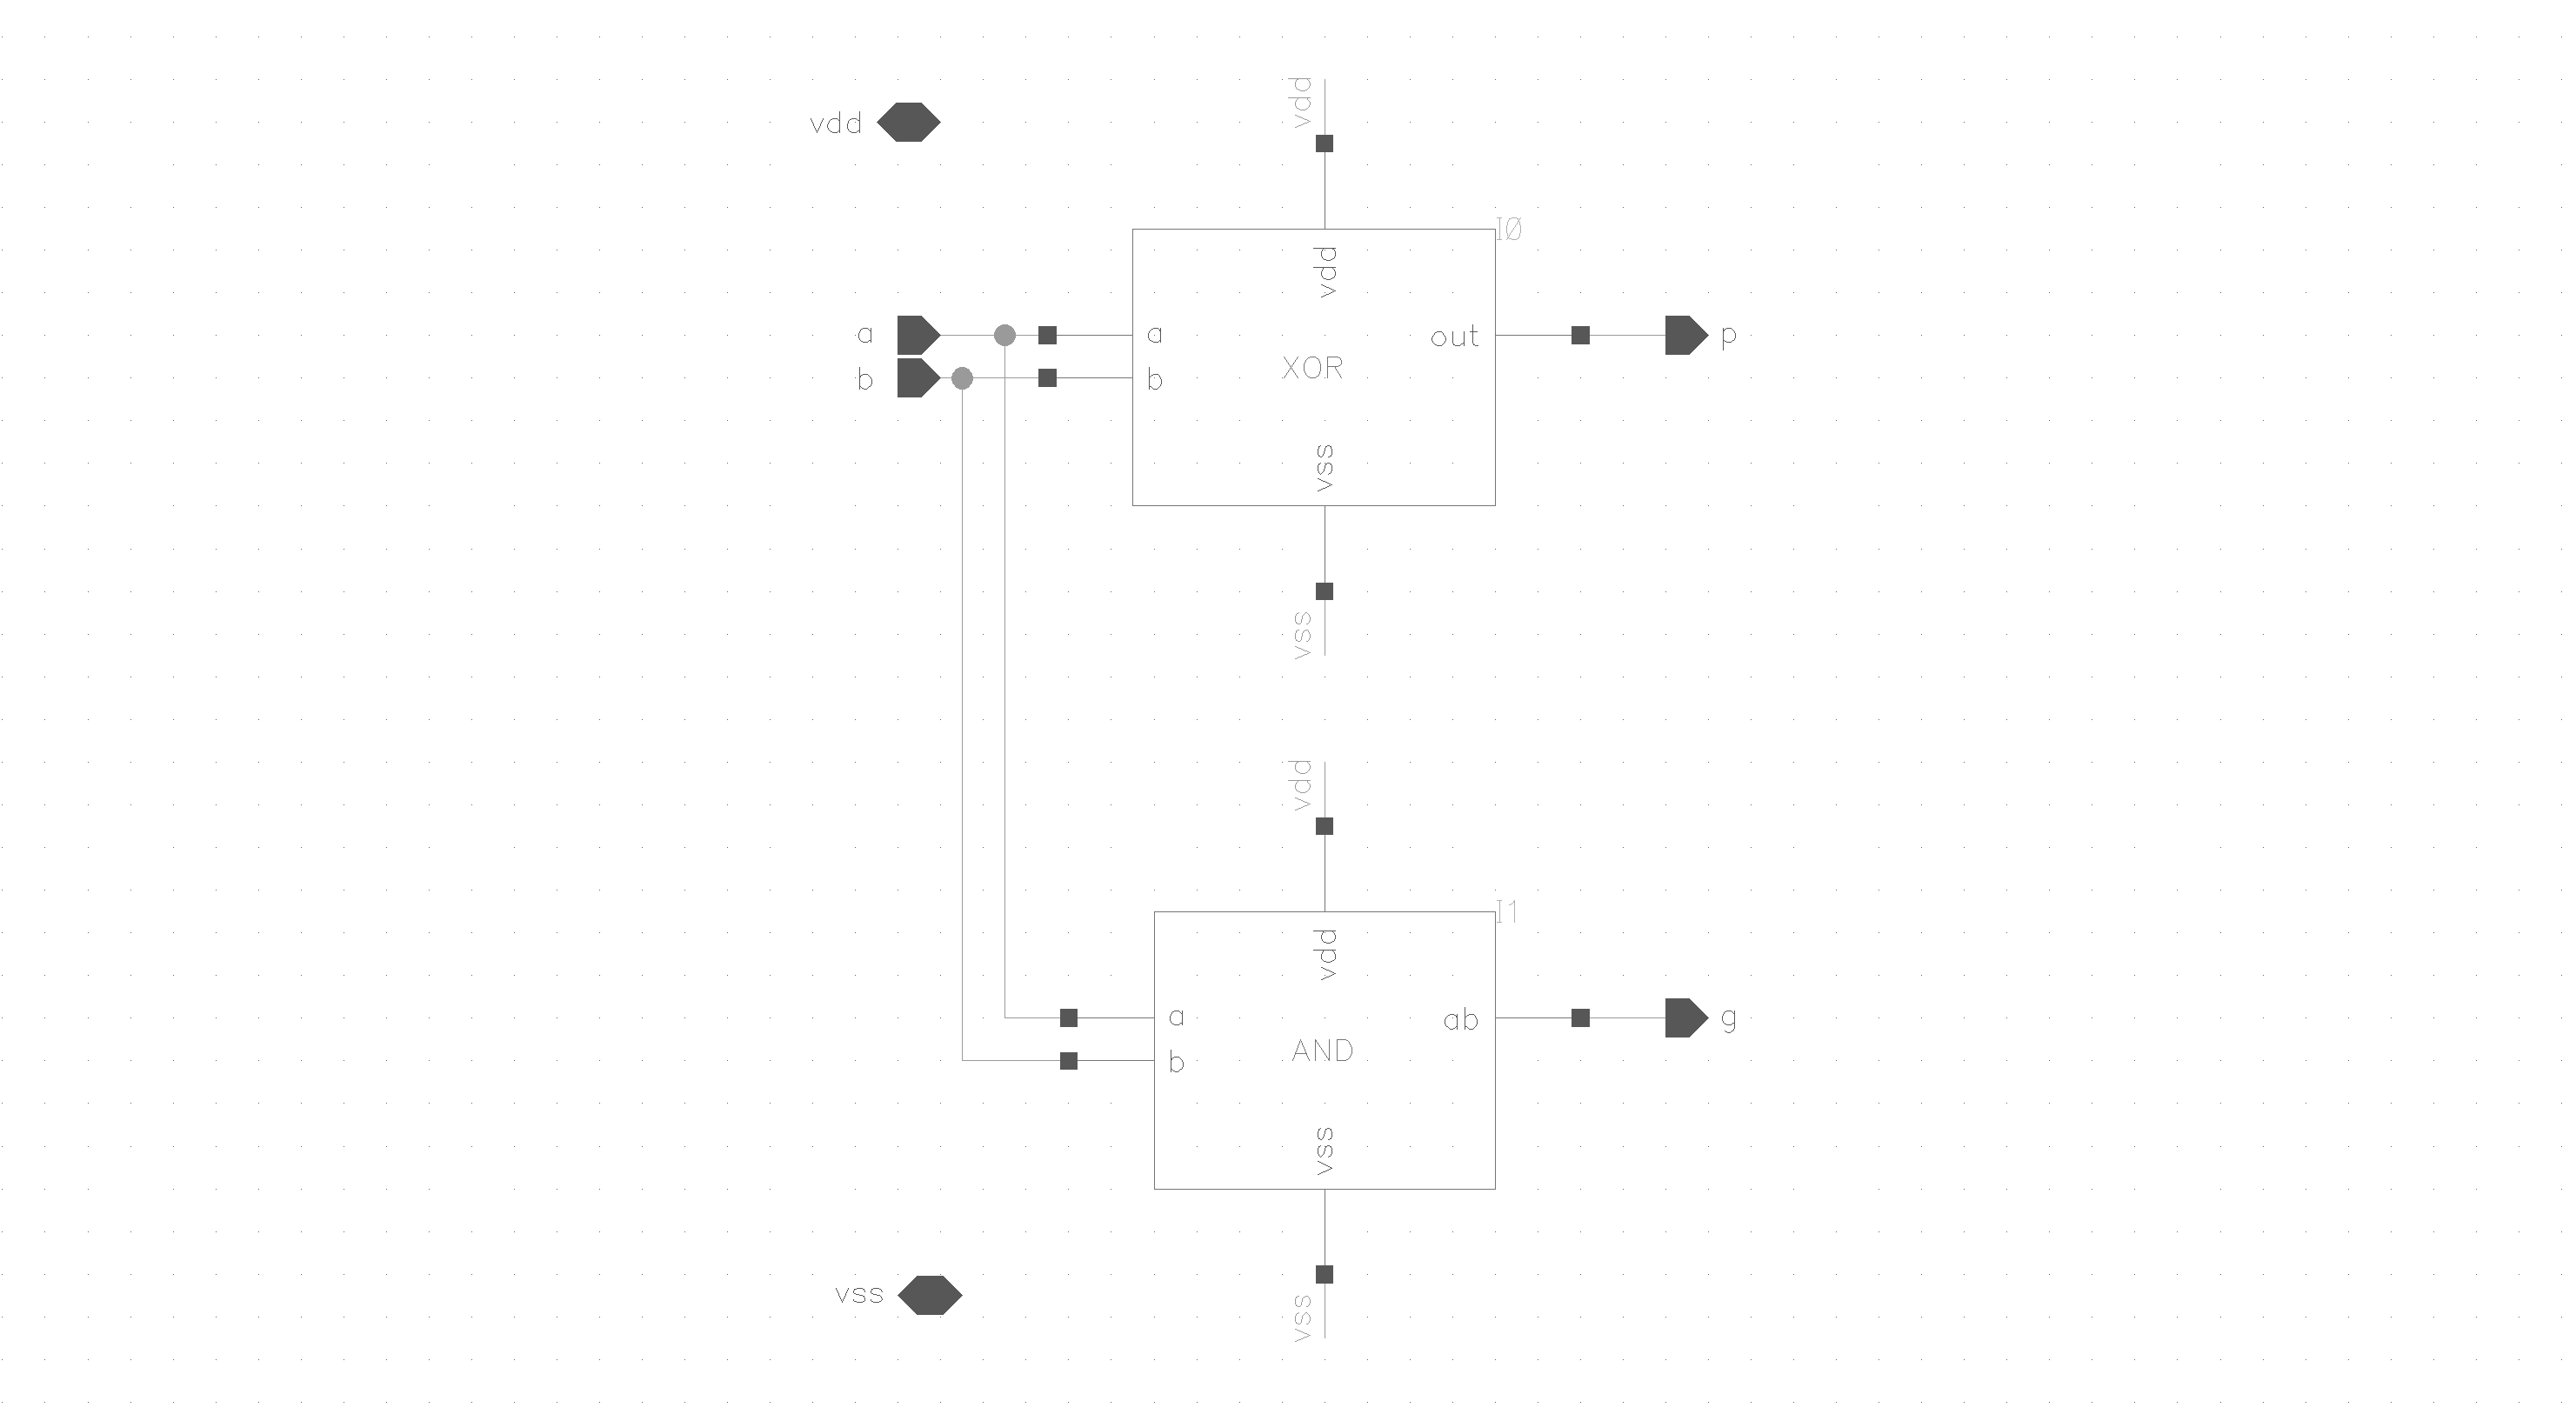
\includegraphics[width=2.0\textwidth]{../figures/red}}
  \caption{Schematic view of the red block.} \label{fig:red}
\end{figure}

\subsubsection{Yellow}

\begin{table}[H]
  \caption{Logic table of yellow block.}
  \centering
  \begin{tabular}{cccc|cc}
    \toprule
    $G_i$ & $G_{i,prev}$ & $P_i$ & $P_{i,prev}$ & $P=P_i \wedge P_{i,prev}$ & $G=(P_i \wedge G_{i,prev}) \vee G_i$ \\
    \midrule
    0 & 0 & 0 & 0 & 0 & 0 \\
    0 & 0 & 0 & 1 & 0 & 0 \\
    0 & 0 & 1 & 0 & 0 & 0 \\
    0 & 0 & 1 & 1 & 1 & 0 \\
    0 & 1 & 0 & 0 & 0 & 0 \\
    0 & 1 & 0 & 1 & 0 & 0 \\
    0 & 1 & 1 & 0 & 0 & 1 \\
    0 & 1 & 1 & 1 & 1 & 1 \\
    1 & 0 & 0 & 0 & 0 & 1 \\
    1 & 0 & 0 & 1 & 0 & 1 \\
    1 & 0 & 1 & 0 & 0 & 1 \\
    1 & 0 & 1 & 1 & 1 & 1 \\
    1 & 1 & 0 & 0 & 0 & 1 \\
    1 & 1 & 0 & 1 & 0 & 1 \\
    1 & 1 & 1 & 0 & 0 & 1 \\
    1 & 1 & 1 & 1 & 1 & 1 \\
    \bottomrule
    \label{tab:yellow}
  \end{tabular}
\end{table}

\begin{figure}[H]
  \centering
  \captionsetup{justification=centering}
  \adjustbox{trim={.15\width} {0\height} {.12\width} {0\height},clip}
  {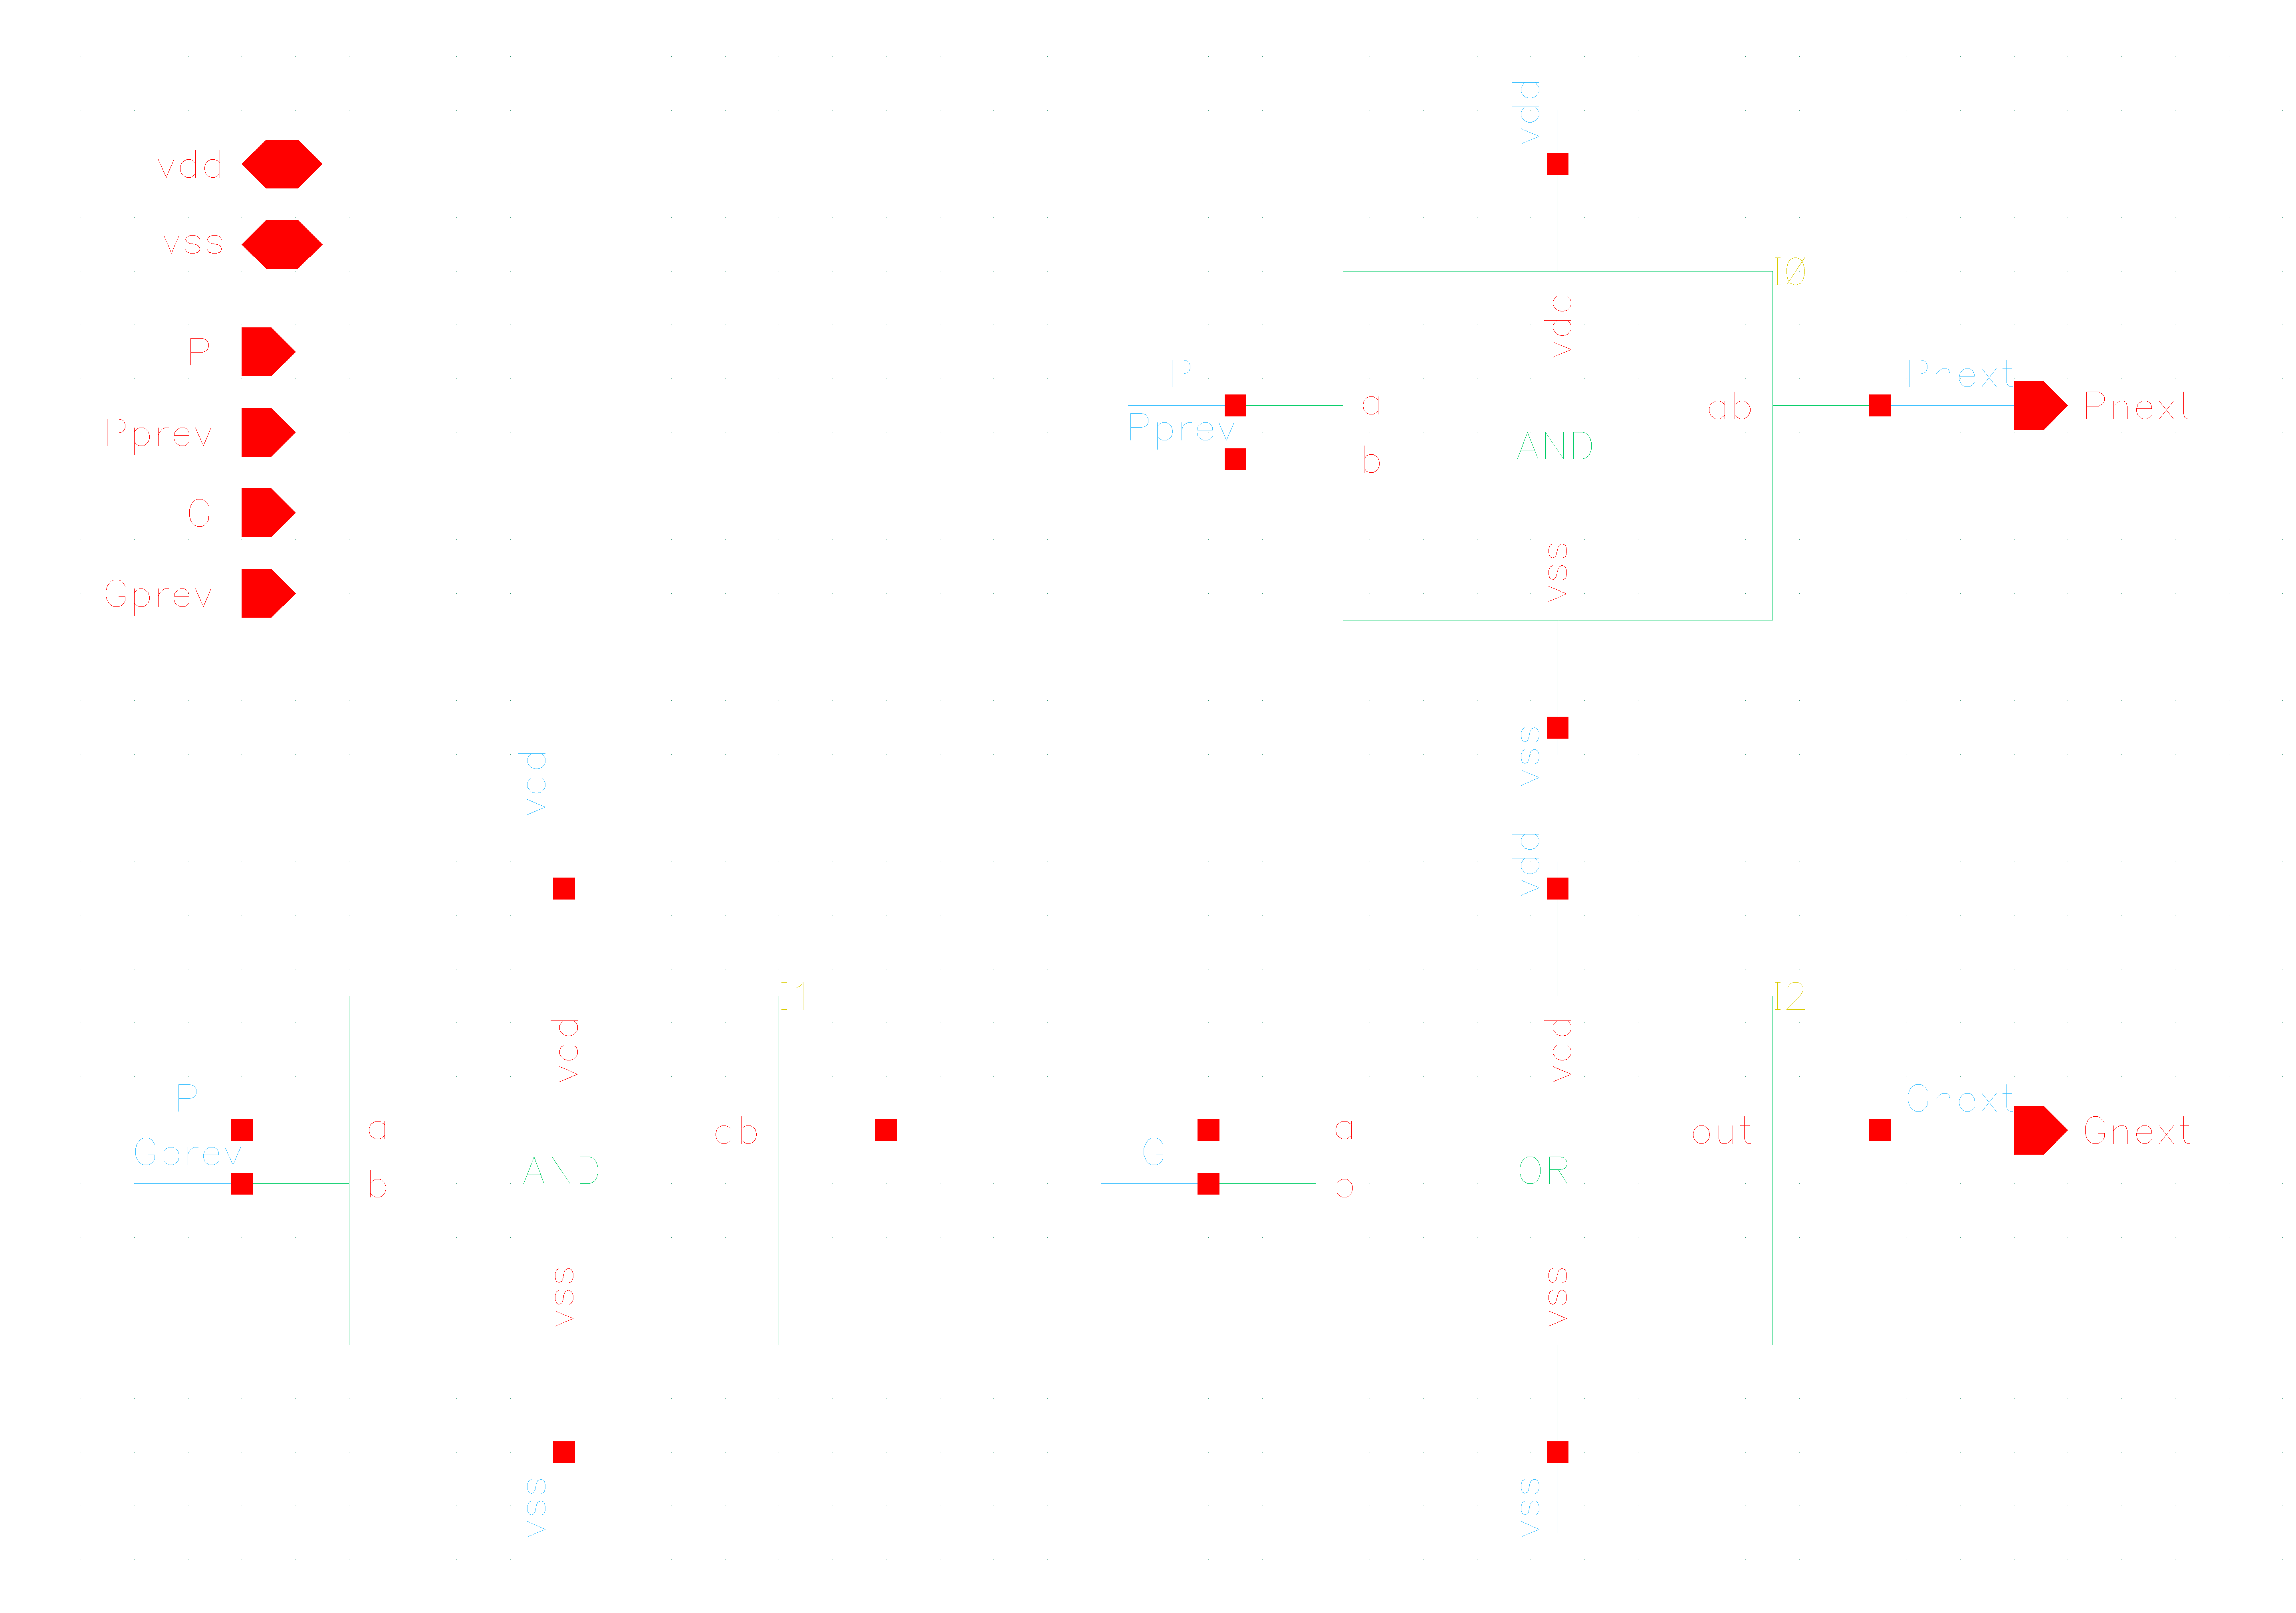
\includegraphics[width=1.3\textwidth]{../figures/yellow}}
  \caption{Schematic view of the yellow block.} \label{fig:yellow}
\end{figure}

\subsubsection{Yellow with carry}

\begin{table}[H]
  \caption{Logic table of yellow with carry block.}
  \centering
  \begin{tabular}{ccc|c}
    \toprule
    $P_i$ & $G_i$ & $G_{i,prev}$ & $G=(P_i \wedge G_{i,prev}) \vee G_i$  \\
    \midrule
    0 & 0 & 0 & 0 \\
    0 & 0 & 1 & 0 \\
    0 & 1 & 0 & 1 \\
    0 & 1 & 1 & 1 \\
    1 & 0 & 0 & 0 \\
    1 & 0 & 1 & 1 \\
    1 & 1 & 0 & 1 \\
    1 & 1 & 1 & 1 \\
    \bottomrule
    \label{tab:yellowcarry}
  \end{tabular}
\end{table}

\begin{figure}[H]
  \centering
  \captionsetup{justification=centering}
  \adjustbox{trim={.1\width} {0\height} {.1\width} {.4\height},clip}
  {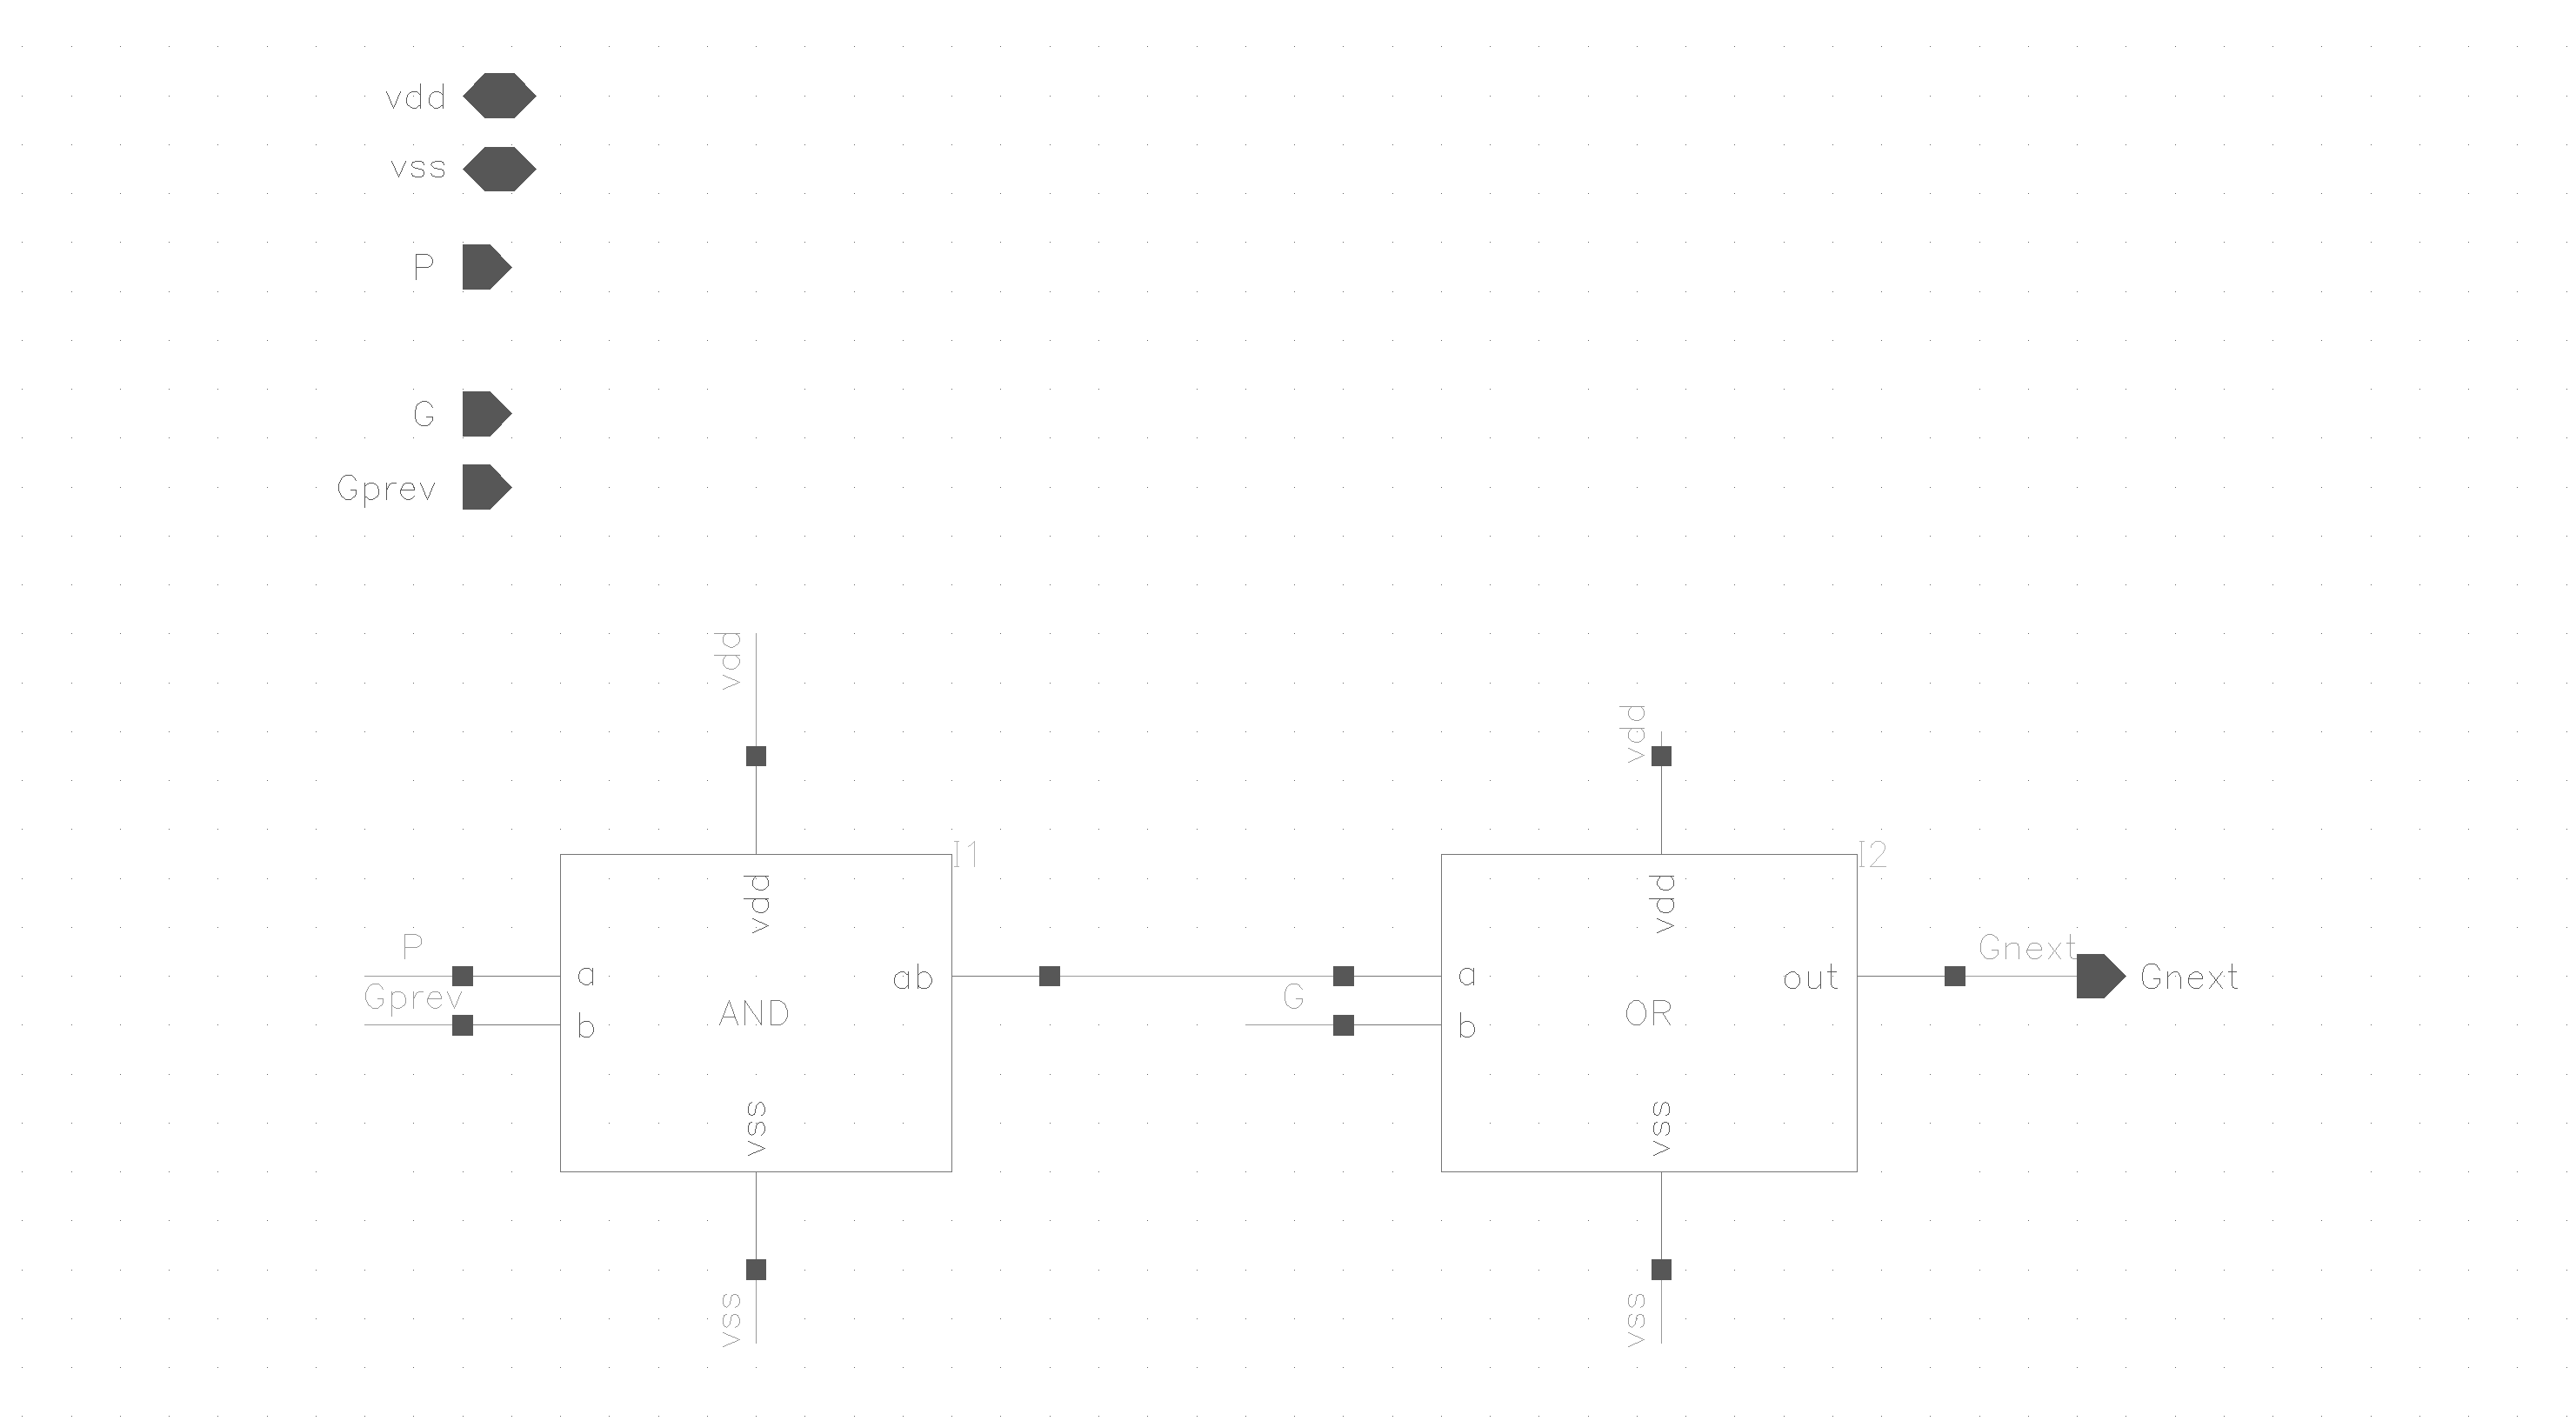
\includegraphics[width=1.2\textwidth]{../figures/yellow_carry}}
  \caption{Schematic view of the yellow carry block.} \label{fig:yellow_c}
\end{figure}

\subsubsection{Sum}

\begin{table}[H]
  \caption{Logic table of sum block.}
  \centering
  \begin{tabular}{cc|c}
    \toprule
    $P_i$ & $C_{i-1}$ & $S_i=P_i \oplus C_{i-1}$ \\
    \midrule
    0 & 0 & 0 \\
    0 & 1 & 1 \\
    1 & 0 & 1 \\
    1 & 1 & 0 \\
    \bottomrule
    \label{tab:sum}
  \end{tabular}
\end{table}

\begin{figure}[H]
  \centering
  \captionsetup{justification=centering}
  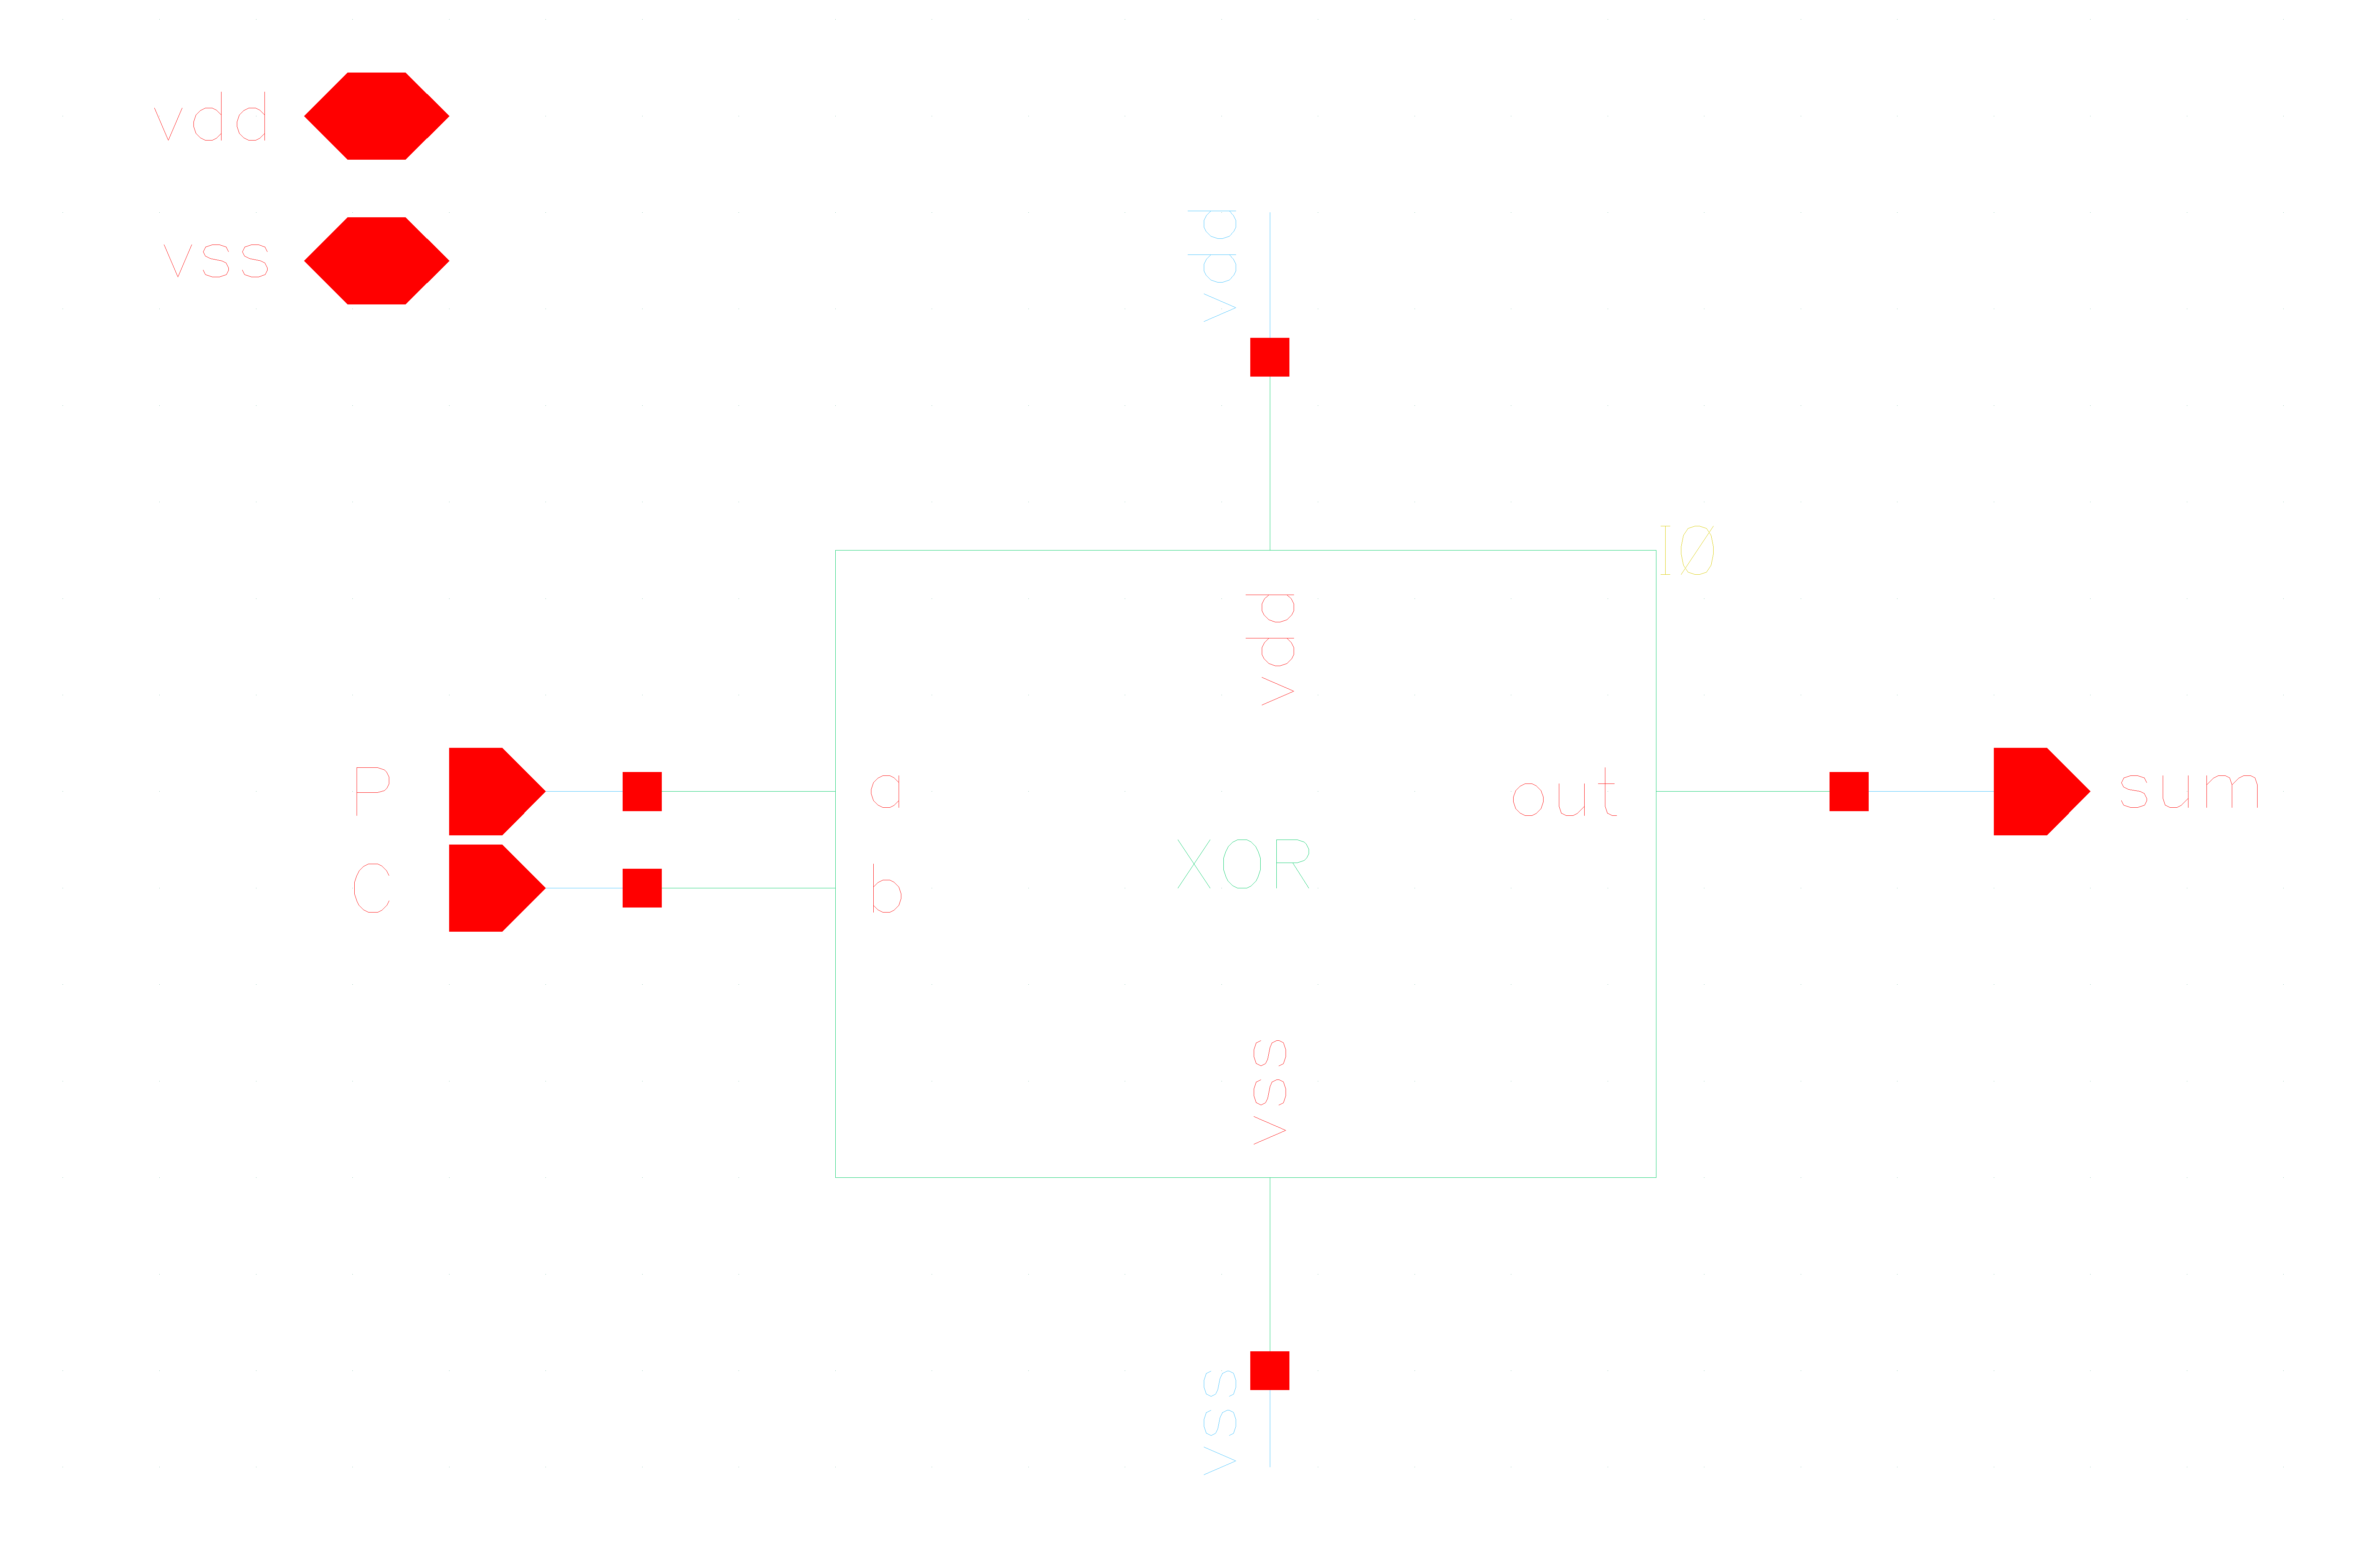
\includegraphics[clip,width=1.0\textwidth]{../figures/sum}
  \caption{Schematic view of the sum block.} \label{fig:sum}
\end{figure}

\subsection{Comparator}
\begin{table}[H]
  \caption{Logic table of XNOR block.}
  \centering
  \begin{tabular}{cc|c}
    \toprule
    $A_i$ & $B_i$ & $Y = \overline{(A_i \oplus B_i)}$ \\
    \midrule
    0 & 0 & 1 \\
    0 & 1 & 0 \\
    1 & 0 & 0 \\
    1 & 1 & 1 \\
    \bottomrule
    \label{tab:xnor}
  \end{tabular}
\end{table}
